\documentclass[12pt,a4paper]{article}
\usepackage{cmap} % Makes the PDF copiable. See http://tex.stackexchange.com/a/64198/25761
\usepackage[T1]{fontenc}
\usepackage[brazil]{babel}
\usepackage[utf8]{inputenc}
\usepackage{amsmath}
\usepackage{amsfonts}
\usepackage{amssymb}
\usepackage{amsthm}
\usepackage{textcomp} % \degree
\usepackage{gensymb} % \degree
\usepackage[usenames,svgnames,dvipsnames]{xcolor}
\usepackage{hyperref}
\usepackage{multicol}
\usepackage{graphicx}
\usepackage[margin=2cm]{geometry}
\usepackage{systeme}

\hypersetup{
    colorlinks = true,
    allcolors = {blue}
}

% TODO: Consider using exsheets
% http://linorg.usp.br/CTAN/macros/latex/contrib/exsheets/exsheets_en.pdf
%
% http://ctan.org/tex-archive/macros/latex/contrib/exercise/
% Options: answerdelayed,lastexercise,noanswer
\usepackage[answerdelayed,lastexercise]{exercise}

\addto\captionsbrazil{%
\def\listexercisename{Lista de exerc\'icios}%
\def\ExerciseName{Exerc\'icio}%
\def\AnswerName{Solu\c{c}\~ao do exerc\'icio}%
\def\ExerciseListName{Ex.}%
\def\AnswerListName{Solu\c{c}\~ao}%
\def\ExePartName{Parte}%
\def\ArticleOf{de\ }%
}

\renewcommand{\ExerciseHeaderTitle}{(\ExerciseTitle)\ }
\renewcommand{\ExerciseListHeader}{%\ExerciseHeaderDifficulty%
\textbf{%\ExerciseListName\
\ExerciseHeaderNB.\ %
%\ --- \
\ExerciseHeaderTitle}%
%\ExerciseHeaderOrigin
\ignorespaces}
\renewcommand{\AnswerListHeader}{\textbf{\ExerciseHeaderNB.\ (\AnswerListName)\ }}

\newcommand{\fixme}{{\color{red}(...)}}
\newcommand*\R{\mathbb{R}}

% Loop Space / CC BY-SA-3.0 / https://tex.stackexchange.com/a/2238/25761
\newenvironment{amatrix}[1]{%
  \left[\begin{array}{@{}*{#1}{c}|c@{}}
}{%
  \end{array}\right]
}

% Loop Space / CC BY-SA-3.0 / https://tex.stackexchange.com/a/3164/25761
%--------grstep
% For denoting a Gauss' reduction step.
% Use as: \grstep{\rho_1+\rho_3} or \grstep[2\rho_5 \\ 3\rho_6]{\rho_1+\rho_3}
\newcommand{\grstep}[2][\relax]{%
   \ensuremath{\mathrel{
       {\mathop{\longrightarrow}\limits^{#2\mathstrut}_{
                                     \begin{subarray}{l} #1 \end{subarray}}}}}}

\renewcommand{\theenumi}{\alph{enumi}}
\renewcommand\labelenumi{(\theenumi) }

\newcommand*\tipo{Prova III (2ª chamada)}
\newcommand*\turma{PRO112-02U}
\newcommand*\disciplina{ALI0001}
\newcommand*\eu{Helder G. G. de Lima}
\newcommand*\data{27/06/2017}

\author{\eu}
\title{\tipo - \disciplina}
\date{\data}

\begin{document}
\thispagestyle{empty}
\newgeometry{margin=2cm,bottom=0.5cm}
\begin{center}

\includegraphics[width=9.0cm]{marca} \\
\textbf{\tipo\ (\disciplina / \turma)} \\
Prof. \eu\footnote{
Este é um material de acesso livre distribuído sob os termos da licença \href{https://creativecommons.org/licenses/by-sa/4.0/deed.pt_BR}{Creative Commons Atribuição-CompartilhaIgual 4.0 Internacional}}
\end{center}

\noindent Nome do(a) aluno(a): \underline{\hspace{9,7cm}} Data: \underline{\data}

%\section*{Instruções}
\begin{center}\fbox{
\begin{minipage}{14cm}

{\footnotesize
\begin{itemize}
\renewcommand{\theenumi}{\Roman{enumi}}
\item Identifique-se em todas as folhas.
\item Mantenha o celular e os demais equipamentos eletrônicos desligados durante a prova.
\item Resolva (integralmente) apenas os itens de que precisar para somar 10,0 pontos.
\end{itemize}
}

\end{minipage}
}
\end{center}

\section*{Questões}
\begin{ExerciseList}
\Exercise[title={2,5}] Seja $\alpha = \left\{
\begin{bmatrix}
0 & 6 \\ 6 & 0
\end{bmatrix},
\begin{bmatrix}
4 & 0 \\ 0 & 4
\end{bmatrix},
\begin{bmatrix}
1 & 0 \\ 0 & -1
\end{bmatrix}
\right\}$ uma base de um subespaço de $M_{2 \times 2}$ e assuma que $\beta = \{A, B, C\}$ é uma outra base do mesmo subespaço, tal que $[I]^\alpha_\beta = \begin{bmatrix}
0 & 2 & 2 \\ 3 & 0 & 3 \\ 0 & 0 & 1
\end{bmatrix}$ é a matriz de mudança da base $\alpha$ para a base $\beta$.
\begin{enumerate}
\item Se $D \in M_{2 \times 2}$ é tal que $[D]_\beta = \begin{bmatrix}
14 \\ 21 \\ 7
\end{bmatrix}$, obtenha $[D]_\alpha$.
\item Determine os vetores (matrizes) $A$, $B$ e $C$ desta base $\beta$.
\end{enumerate}
\Answer \fixme

\Exercise[title={2,5}] Verifique se há algum operador linear $T:\R^2 \to \R^2$ que transforma a figura $S$ na figura $S'$ conforme mostrado a seguir. Em caso afirmativo, obtenha $T(x,y)$. Apresente argumentos teóricos que comprovem sua resposta.
\begin{center}
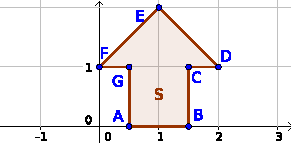
\includegraphics[width=7.0cm]{img/prova-3-pro-plano-1}
\hspace{1cm}
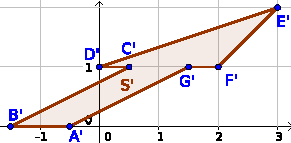
\includegraphics[width=7.0cm]{img/prova-3-pro-plano-2}
\end{center}
\Answer \fixme

\Exercise[title={2,5}] Suponha que $T_1: \R^2 \to P_2$ e $T_2: P_2 \to P_1$ sejam transformações lineares.
\begin{enumerate}
\item Assumindo que $T_1$ e $T_2$ sejam injetoras, o que se pode concluir sobre a injetividade da composta $T_2 \circ T_1$? Prove que a sua conclusão está correta.
\item Mostre que se $T_1(a,b) = ax^2 + bx$ e $T_2(q(x)) = q^\prime(x)$, então $T_2 \circ T_1$ é um isomorfismo.
\end{enumerate}
\Answer \fixme

\Exercise[title={2,5}] Seja $R: \R^2 \to \R^2$ a transformação linear que rotaciona os vetores de $\R^2$ em torno da origem segundo um ângulo $\pi/2$ no sentido anti-horário. Considere também a transformação linear $S: \R^2 \to \R^2$ que faz a reflexão em relação ao eixo $y$. Mostre que $R^{-1} \circ S = S \circ R$.
\Answer \fixme

\Exercise[title={2,5}] Se $L: M_{2 \times 2} \to M_{2 \times 2}$ é o operador linear definido por $L(X) = X - X^T$, obtenha $N(L)$ e $\operatorname{Im}(L)$. Levando em conta os subespaços que encoutrou, pode-se dizer que $L$ é bijetora?
\Answer \fixme
\end{ExerciseList}

\begin{center}
BOA PROVA!
\end{center}

%\newpage
%\restoregeometry
%\section*{Respostas}
%\shipoutAnswer
\end{document}
